\chapter{Adding}

In this model, we found 2 flavors of period-adding structures.
The first one is period adding in between the chains of the same period.
The other is period adding near ``type B'' period regions.

\section{Adding in Between Chains of the Same Period}

\Cref{fig:minrep.adding1.overview} shows both the periods of the model initially, as described in the previous chapter (\Cref{chap:minrep}), as well as the model with period-adding structures.
For \Cref{fig:minrep.adding1.overview.adding}, only the values of the fixed parameters $a_L = 1, b_L = 0.5$ are changed.
Initially, the values for these parameters were $a_L = 4, b_L = -0.5$.
The only other fixed parameter $B$ stays the same and the parameter ranges of $p_x$ and $p_y$ were adjusted slightly.
That means, that the shape of the function only changed on the branches $f_{\A}$ and $f_{\C}$.

When comparing both figures, we can see that there are no ``type B'' period regions in \Cref{fig:minrep.adding1.overview.adding}, the period-adding situation.
Instead, it looks like the ``type A'' period regions of the same period overlap now.
Also, the regions of higher periods in between the chains are new, these are the period-adding regions.
At the points, where these regions make a turn, there are period regions of even higher periods.
The meaning of these is explored in a later section, the next section will focus on the disappearance of the ``type B'' parameter regions.

\begin{figure}
    \centering
    \subfloat[Initial situation]{
        \includegraphics[width=.5 \textwidth]{62_MinimalRepr_Adding/2D_Period_4/result.png}
    }
    \subfloat[Period-adding]{
        \includegraphics[width=.5 \textwidth]{62_MinimalRepr_Adding/2D_Period_1/result.png}
        \label{fig:minrep.adding1.overview.adding}
    }
    \caption{Overview of period-adding structures in between chains of the same period}
    \label{fig:minrep.adding1.overview}
\end{figure}

\subsection{Disappearance of ``Type B'' Parameter Regions}
\label{sec:minrep.adding.disapp.typeB}

\Cref{fig:minrep.path.to.disappearance} shows diagrams depicting the borders of parameter regions of specific stable cycles.
The lower left corner of the diagrams is always in the period region with the stable cycle $\Cycle{\A^7\B^3\C^7\D^3}$, the cycles in the upper left ($\Cycle{\A^6\B^3\C^6\D^3}$), upper right ($\Cycle{\A^6\B^4\C^6\D^4}$), lower right ($\Cycle{\A^7\B^4\C^7\D^4}$), and middle ($\Cycle{\A^7\B^3\C^6\D^4}$ and $\Cycle{\A^6\B^4\C^7\D^3}$) follow.
The diagrams show the evolution of the ``type B'' parameter region along a line in the parameter space from $a_L = 4, b_L = -0.5$ to $a_L = 1, b_L = 0.5$.
This line is given by the equation $a_L = \frac{5}{2} - 3 \cdot b_L$.

The first thing that happens is shown in \Cref{fig:minrep.path.to.disappearance.1}.
``Type A'' parameter regions stop overlapping with the ``type A'' period regions above, but only on the left side.
This effect is illustrated by the lower and upper right parameter regions in the diagram.
All other overlaps remain, but they are a lot smaller, especially the overlaps of the ``type B'' parameter region in the middle with the surrounding ``type A'' parameter regions.
In the space between the lower and upper right ``type A'' parameter regions, period adding emerges.

In the next diagram, \Cref{fig:minrep.path.to.disappearance.2}, the lower left ``type A'' parameter region starts overlapping with the upper right ``type A'' parameter region.
At the same time, this overlap will make the ``type B'' parameter region in the middle smaller, it doesn't exist in the new overlapping area anymore.
This overlap is completed in \Cref{fig:minrep.path.to.disappearance.3} and the ``type B'' parameter region disappears completely.
At this point, the upper left and upper right parameter regions stop overlapping and in the space between those two parameter regions, period adding emerges.
The same also happens to the lower left and lower right parameter regions.
The lower left and upper left parameter regions still overlap on the right side.

This last remaining overlap of ``type A'' parameter regions, that existed for the initial situation disappears with \Cref{fig:minrep.path.to.disappearance.3}.
Here only the lower left and upper right ``type A'' parameter regions overlap and between all other ``type A'' parameter regions there is space with period adding.
In the corners of these period-adding regions, we can notice rectangular structures.
The next section will explore this phenomenon.



\begin{figure}
    \centering
    \subfloat[$a_L = 2.8, b_L = -0.1$]{
        \includegraphics[width=.5 \textwidth]{62_MinimalRepr_Adding/2D_Regions_2.8/Manual/result.png}
        \label{fig:minrep.path.to.disappearance.1}
    }
    \subfloat[$a_L = 2.725, b_L = -0.075$]{
        \includegraphics[width=.5 \textwidth]{62_MinimalRepr_Adding/2D_Regions_2.725/Manual/result.png}
        \label{fig:minrep.path.to.disappearance.2}
    } \\
    \subfloat[$a_L = 2.65, b_L = -0.05$]{
        \includegraphics[width=.5 \textwidth]{62_MinimalRepr_Adding/2D_Regions_2.65/Manual/result.png}
        \label{fig:minrep.path.to.disappearance.3}
    }
    \subfloat[$a_L = 2.5, b_L = 0$]{
        \includegraphics[width=.5 \textwidth]{62_MinimalRepr_Adding/2D_Regions_2.5/Manual/result.png}
        \label{fig:minrep.path.to.disappearance.4}
    }
    \caption{Evolution of ``type B'' parameter regions when transitioning to a period adding scenario}
    \label{fig:minrep.path.to.disappearance}
\end{figure}

\subsubsection{``Type B'' Cycles Just Before Disappearing}

Just before the ``type B'' period region disappears, at $a_L = 2.675, b_L = -0.58\overline{3}$, the cycles that exist there are extremely close to colliding with 3 different borders each.
\Cref{fig:minrep.just.before.disappearance.cob} shows the cobweb diagram of the cycles.
Both cycles are so close to each other on branches $f_\A$ and $f_\B$, that we can't tell them apart.
Even in the vastly enhanced blowup plot in the upper left corner of the figure, both cycles are almost on top of each other.
At the boundary $d_1$ the cycles split, because of the symmetry the same happens at $d_3$ again.
At $d_1$, the cycle $\Cycle{\A^7\B^3\C^6\D^4}$ (green) is mapped onto $f_\A$ one last time, while its twin cycle $\Cycle{\A^6\B^4\C^7\D^3}$ (brown) is directly mapped to $f_\B$.
At $d_3$, the same thing happens, but the two cycles are swapped.

As for the cycles near $d_0$ and $d_2$, the cycle $\Cycle{\A^7\B^3\C^6\D^4}$ is next to $d_2$, while its twin cycle is near $d_0$.
The collision of the cycles with the borders at the same time corresponds to the right boundary of the ``type B'' period region.
This follows from \Cref{sec:minrep.bif}, where all bifurcations in this model are listed and explained.
The two bifurcations are denoted as $\BCB_{d_0}^{\A^6\B^4\C^7\D^3, r}$ and $\BCB_{d_2}^{\A^7\B^3\C^6\D^4, r}$.
As this boundary does not move as much as the other two still existing boundaries when transitioning to the period adding scenario, this bifurcation is not as important to us now.

The cycles near $d_1$ and $d_3$ correspond to the upper and lower boundaries of the ``type B'' period region.
Again, the correspondence follows from \Cref{sec:minrep.bif}.
The upper and lower boundaries of ``type B'' period regions are border collision bifurcations where the two cycles collide with $d_1$ and $d_3$ at the same time, one cycle with one boundary each.
For the upper boundary, the cycle with more points on the branch $f_\A$ collides with the border $d_3$ from the left, denoted as $\BCB_{d_3}^{\A^7\B^3\C^6\D^4, l}$.
Its twin cycle collides with $d_1$, also from the left.
This follows from the symmetry and is denoted as $\BCB_{d_1}^{\A^6\B^4\C^7\D^3, l}$.
For the lower boundary, now the cycles collide from the right instead of the left, but the borders with which each cycle collides stay the same.
So for this boundary we have the bifurcations $\BCB_{d_3}^{\A^7\B^3\C^6\D^4, l}$ and $\BCB_{d_1}^{\A^6\B^4\C^7\D^3, r}$.
These two boundaries get closer to each other as we lower $a_L$ as we can see in \Cref{sec:minrep.adding.disapp.typeB}.

\begin{figure}
    \centering
    \subfloat[Regions]{
        \includegraphics[width=.3 \textwidth]{62_MinimalRepr_Adding/2D_Regions_2.675/Manual/result.png}
        \label{fig:minrep.just.before.disappearance.reg}
    }
    \subfloat[Cobweb at point $A$]{
        \includegraphics[width=.3 \textwidth]{62_MinimalRepr_Adding/Cob_2.675_A/Manual/result.png}
        \label{fig:minrep.just.before.disappearance.cob}
    }
    \subfloat[Cobweb at point $B$]{
        \includegraphics[width=.3 \textwidth]{62_MinimalRepr_Adding/Cob_2.675_B/Manual/result.png}
        \label{fig:minrep.just.before.disappearance.cob}
    }
    \label{fig:minrep.just.before.disappearance}
    \caption{bla}
\end{figure}
